\documentclass{beamer}

\usepackage{listings}
\usepackage[utf8]{inputenc}
\usepackage{color}
\usepackage{tikz}
\usetikzlibrary{shapes.callouts,decorations.pathmorphing}

\author{Attila Nagy}
\date{March 10, 2014}
\title{Design Patterns}
\subtitle{Singletons, Pools and Factories}
\usetheme{CambridgeUS}

\definecolor{mygreen}{rgb}{0,0.6,0}
\definecolor{mygray}{rgb}{0.5,0.5,0.5}
\definecolor{mymauve}{rgb}{0.58,0,0.82}
\definecolor{myyellow}{rgb}{0.8,0.8,0}

\lstset{
basicstyle=\footnotesize,
breakatwhitespace=false,
breaklines=true,
captionpos=b,
commentstyle=\color{mygreen},
deletekeywords={...},
escapeinside={\%*}{*)},
extendedchars=true,
emph={nullptr},
emphstyle={\color{red}},
frame=single,
keepspaces=true,
keywordstyle=\color{blue},
language=C++,
morekeywords={*,...,},
numbers=left,
numbersep=5pt,
numberstyle=\tiny\color{mygray},
rulecolor=\color{black},
showspaces=false,
showstringspaces=false,
showtabs=false,
stepnumber=1,
stringstyle=\color{mymauve},
tabsize=2,
title=\lstname
}

\newcommand{\popup}[1]{
\begin{tikzpicture}[overlay,remember picture]
  \pgftransformshift{\pgfpointanchor{current page}{center}}
  \node[
    ellipse callout,
    draw=red,
    ultra thick,
    fill=yellow,
    decoration=zigzag,
    decorate,
    callout relative pointer=(225:0cm),
    font=\Huge,
    text width=0.6\textwidth,
    align=center,
    anchor=center
  ] at (0,0) {#1};
\end{tikzpicture}
}

\begin{document}

\defverbatim[colored]\simpleSingleton{\scriptsize
\begin{lstlisting}[language=C++,basicstyle=\ttfamily,mathescape]
class Singleton {
public:
static Singleton& getInstance() {
  if (nullptr == pInstance) {
    pInstance = new Singleton;
  }
  return *pInstance;
}

private:
Singleton () = default;
Singleton (const Singleton&) = delete;
Singleton operator= (const Singleton&) = delete;
$\sim$Singleton () = delete;

static Singleton* pInstance;
// More Functions and Data
};
Singleton* Singleton::pInstance = nullptr;
\end{lstlisting}
}

\defverbatim[colored]\meyersSingleton{\scriptsize
\begin{lstlisting}[language=C++,basicstyle=\ttfamily,mathescape]
class Singleton {
public:
static Singleton& getInstance() {
  static Singleton instance;
  return instance;
}

private:
Singleton () = default;
Singleton (const Singleton&) = delete;
Singleton operator= (const Singleton&) = delete;
$\sim$Singleton () = default;

// More Functions and Data
};
\end{lstlisting}
}

\defverbatim[colored]\deadReference{\scriptsize
\begin{lstlisting}[language=C++,basicstyle=\ttfamily,mathescape]
class Singleton {
public:
static Singleton& getInstance() {
  static Singleton instance;
  if (destroyed) {
    throw std::runtime_error("Dead Reference");
  }
  return instance;
}
private:
Singleton () = default;
Singleton (const Singleton&) = delete;
Singleton operator= (const Singleton&) = delete;
$\sim$Singleton (){
  destroyed = true;
}

static bool destroyed;
// More Functions and Data
};
bool Singleton::destroyed = false;
\end{lstlisting}
}

\defverbatim[colored]\phoenixSingleton{\tiny
\begin{columns}[t]
  \begin{column}{.47\textwidth}
\begin{lstlisting}[language=C++,basicstyle=\ttfamily,mathescape]
class Singleton {
public:
static Singleton& getInstance() {
  if (destroyed) {
    new(pInstance) Singleton;
    atexit(KillSingleton);
  }
  if (nullptr == pInstance) {
    static Singleton instance;
    pInstance = &instance;
  }
  return *pInstance;
}
static void KillSingleton(void) {
  pInstance->$\sim$Singleton();
}
\end{lstlisting}
  \end{column}
  \begin{column}{.47\textwidth}
    \lstset{firstnumber=last}
\begin{lstlisting}[language=C++,basicstyle=\ttfamily,mathescape]
private:
Singleton () {
  destroyed = false;
}
Singleton (const Singleton&) = delete;
Singleton operator= (const Singleton&) = delete;
$\sim$Singleton () {
  destroyed = true;
  pInstance = nullptr;
}
static bool destroyed;
static Singleton* pInstance;
};
bool Singleton::destroyed = false;
Singleton* Singleton::pInstance = nullptr;
\end{lstlisting}
  \end{column}
\end{columns}
}

\defverbatim[colored]\multithreada{\scriptsize
\begin{lstlisting}[language=C++,basicstyle=\ttfamily,mathescape]
static Singleton& getInstance() {
  if (nullptr == pInstance) {
    pInstance = new Singleton;
  }
  return *pInstance;
}
\end{lstlisting}
}

\defverbatim[colored]\multithreadb{\scriptsize
\begin{lstlisting}[language=C++,basicstyle=\ttfamily,mathescape]
static Singleton& getInstance() {
  Lock guard(mutex);
  if (nullptr == pInstance) {
    pInstance = new Singleton;
  }
  return *pInstance;
}
\end{lstlisting}
}

\defverbatim[colored]\multithreadc{\scriptsize
\begin{lstlisting}[language=C++,basicstyle=\ttfamily,mathescape]
static Singleton& getInstance() {
  if (nullptr == pInstance) {
    Lock guard(mutex);
    pInstance = new Singleton;
  }
  return *pInstance;
}
\end{lstlisting}
}

\defverbatim[colored]\multithreadd{\scriptsize
\begin{lstlisting}[language=C++,basicstyle=\ttfamily,mathescape]
static Singleton& getInstance() {
  if (nullptr == pInstance) {
    Lock guard(mutex);
    if (nullptr == pInstance) {
      pInstance = new Singleton;
    }
  }
  return *pInstance;
}
\end{lstlisting}
}

\begin{frame}
\maketitle{}
\centering{
  {\em https://github.com/NagyAttila/DesignPatterns}
}
\end{frame}


\section{Content}
\begin{frame}{Content}
\begin{itemize}
  \item \Large{Object Oriented Design Principles}
    \vspace{0.25cm}
\begin{columns}
  \hfill
  \begin{column}{.3\textwidth}
    \begin{block}{}
      \begin{itemize}
        \item Singleton
        \item Meyers Singleton
        \item Phoenix Singleton
      \end{itemize}
    \end{block}
  \end{column}
  \begin{column}{.3\textwidth}
    \begin{block}{}
      \begin{itemize}
        \item Object Pool
        \item Connection Pool
        \item Thread Pool
      \end{itemize}
    \end{block}
  \end{column}
  \begin{column}{.3\textwidth}
    \begin{block}{}
      \begin{itemize}
        \item Factory Method
        \item Abstract Factory
        \item Object Factory
      \end{itemize}
    \end{block}
  \end{column}
\end{columns}
\end{itemize}
\end{frame}


\section{Principles}
\begin{frame}{Object Oriented Design Principles}
\begin{block}{Open Close Principle}
  Classes are open for extension but closed for modification.
\end{block}
\pause
\begin{block}{Liskov's Substitution Principle}
  Derived classes extend the base classes without changing their behavior.
\end{block}
\pause
\begin{block}{Dependency Inversion Principle}
  High level classes should depend on abstract classes.
\end{block}
\pause
\begin{block}{Interface Segregation Principle}
  Fat interface avoidance. \\
  Clients should not be forced to depend on interface that they don't use.
\end{block}
\pause
\begin{block}{Single Responsibility Principle}
  One class should be responsible for one thing.
\end{block}
\end{frame}


\section{Singleton}
\begin{frame}{Singleton}
Purpose:
\begin{itemize}
  \item class has at most one instance,
  \item that instance is accessible in a global scope.
\end{itemize}

Application Areas:
\begin{itemize}
  \item logging,
  \item Thread and Connection Pools,
  \item Factories
  \item system clock,
  \item etc.
\end{itemize}
\end{frame}

\begin{frame}{Singleton - How?}
\begin{columns}
  \begin{column}{.3\textwidth}
    \textbullet  private constructors
  \end{column}
  \begin{column}{.6\textwidth}
    \textbullet  static {\em \_pInstance\_} and {\em \_getInstance\_}
  \end{column}
\end{columns}

\simpleSingleton
\uncover<2->{
  \popup{Destructor was never called! (memory leak)}
}
\end{frame}

\begin{frame}{Meyers Singleton}
\textbullet local static {\em \_instance\_}
\meyersSingleton

$\Rightarrow$ private destructor is called at process termination \\

\pause
\popup{Dead Reference!}
\end{frame}

\begin{frame}{Dead Reference Problem}
How?
\begin{enumerate}
  \item<1-> Two Singleton classes, Logger and Keyboard, in different compilation units
  \item<2-> Keyboard uses Logger
  \item<3-> termination: Logger deallocated, Keyboard tries to use it
  \item<4-> Logger's static object "shell" is still available
  \item<5-> {\color{red}undefined behaviour} (probably crash)
\end{enumerate}

\uncover<6->{
  Why?
  \begin{itemize}
    \item order of deallocation of static objects is not deterministic
  \end{itemize}
}

\uncover<7->{
  Solution?
  \begin{itemize}
    \item on-demand reallocation of {\em Singleton} after destruction
  \end{itemize}
}

\uncover<7->{
  \hspace{1cm}$\Rightarrow$ Phoenix Singleton
}
\end{frame}

\begin{frame}{Phoenix Singleton}
\begin{columns}
  \begin{column}{.47\textwidth}
    \begin{block}{Combination of the 3 approaches:}
      \begin{itemize}
        \item Simple: {\em \_pInstance\_} pointer
        \item Meyers: static life-time
        \item Dead Reference: detection
      \end{itemize}
    \end{block}
  \end{column}
  \begin{column}{.47\textwidth}
    \begin{block}{Plus:}
      \begin{itemize}
        \item on-demand reallocation
        \item destructor called using {\em \_atexit\_}
        \item multiple time "reborn"
      \end{itemize}
    \end{block}
  \end{column}
\end{columns}

\phoenixSingleton
\pause

\popup{?`Problem?}
\end{frame}

\begin{frame}{atexit Problem}
Problem:
\begin{itemize}
  \item<1-> functions registered on stack
  \item<2-> last registered called first
  \item<3-> registering from a registered function
  \item<4-> too late to be first
  \item<5-> some old compilers might crash
\end{itemize}

\uncover<5->{
  Solution?
}
\uncover<6->{
  \begin{itemize}
    \item Read the Manual!
    \item Use the newest compilers!
  \end{itemize}
}
\end{frame}


\begin{frame}{Multithreading}
Problem:
\begin{itemize}
  \item general lazy initialization problem
  \item race condition
\end{itemize}

\uncover<2->{Solution:}
\begin{enumerate}[A]
    \item<2-> local static instance (Meyers approach)
    \item<3-> locking
    \item<5-> double-check locking
\end{enumerate}

\only<1-2>{\multithreada}
\only<3>{\multithreadb}
\only<4>{\multithreadc}
\only<5>{\multithreadd}
\end{frame}

\begin{frame}{Notes}
\begin{block}{Why not global?}
  \vspace{-0.4cm}
  \begin{itemize}
      \begin{columns}
        \begin{column}{.3\textwidth}
          \item uniqueness
          \item lack of laziness
          \item pollute global scope
        \end{column}
        \begin{column}{.45\textwidth}
        \item not always possible
          \begin{itemize}
            \item dependency
            \item need data for init
          \end{itemize}
        \end{column}
      \end{columns}
  \end{itemize}
\end{block}

\pause

\begin{block}{Possible extensions and alternative solutions:}
  \begin{itemize}
    \item longevity control for dead reference problem
    \item registry high number of singletons
    \item inheritance
  \end{itemize}
\end{block}

\pause

\begin{block}{Final thought:}
  \vspace{-0.4cm}
  \begin{itemize}
      \begin{columns}
        \begin{column}{.4\textwidth}
          \item should be used sparingly
        \end{column}
        \begin{column}{.4\textwidth}
        \item if needs a lot:
          \begin{itemize}
            \item[$\Rightarrow$] use registry, or
            \item[$\Rightarrow$] change design
          \end{itemize}
        \end{column}
      \end{columns}
  \end{itemize}
\end{block}
\end{frame}


\section{Pools}
\begin{frame}{Object Pool}
\begin{columns}
  \begin{column}{.47\textwidth}

    \begin{block}{Purpose:}
      \begin{itemize}
        \item reuse objects
        \item eliminate object allocation / deallocation overhead
      \end{itemize}
    \end{block}

    \pause

    \begin{block}{Useful when:}
      \begin{itemize}
        \item high instantiation cost
        \item high instantiation rate
        \item low number of concurrently used instances
      \end{itemize}
    \end{block}
  \end{column}

  \pause

  \begin{column}{.47\textwidth}
    \begin{block}{Pitfalls:}
      \begin{itemize}
        \item reset object after use
          \begin{itemize}
            \item[$\Rightarrow$] false authentication
            \item[$\Rightarrow$] information leak
          \end{itemize}
        \item object not released
      \end{itemize}
    \end{block}

    \pause

    \begin{block}{Empty pool:}
      \begin{enumerate}
        \item report error
        \item increase pool size
        \item blocking request
      \end{enumerate}
    \end{block}
  \end{column}
\end{columns}

\pause

\begin{columns}
  \begin{column}{.47\textwidth}
    \begin{block}{Similar patterns}
      \begin{itemize}
        \item Connection Pool
        \item Thread Pool
      \end{itemize}
    \end{block}
  \end{column}

  \begin{column}{.47\textwidth}
    \begin{block}{Used as}
      \begin{itemize}
        \item Singleton
      \end{itemize}
    \end{block}
  \end{column}
\end{columns}

\end{frame}

\begin{frame}{Connection Pool and Thread Pool}
\vspace{-0.25cm}
\begin{block}{Connection Pool}
  \begin{itemize}
    \item cache of DB connections
    \item creates new connection if empty pool (2nd approach)
  \end{itemize}
\end{block}

\vspace{-0.25cm}
\pause

\begin{columns}
  \begin{column}{.47\textwidth}
    \begin{block}{Thread Pool}
      \begin{itemize}
        \item asynchronous task processing
        \item more tasks than threads
        \item fix or dynamic number of threads
      \end{itemize}
    \end{block}
  \end{column}

  \begin{column}{.47\textwidth}
    \begin{figure}[t]
      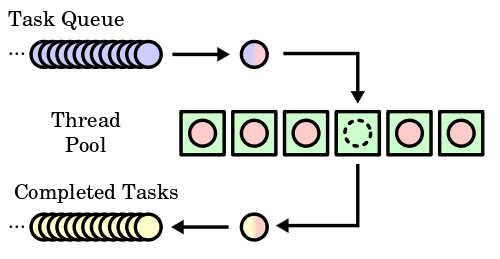
\includegraphics[width=\textwidth]{500px-Thread_pool.png}
    \end{figure}
  \end{column}
\end{columns}

\uncover<2->{
\vspace{-0.25cm}
  \begin{block}{Threads}
    \begin{description}
      \item<2->[too many created $\Rightarrow$] wasting resource and time
      \item<3->[too many destroyed $\Rightarrow$] more time recreating them
      \item<4->[too slow creation $\Rightarrow$] long waiting times at clients
      \item<5->[too slow destroy $\Rightarrow$] wasting resource and time
    \end{description}
  \end{block}
}
\end{frame}


\section{Factories}
\begin{frame}{Factory Method}
  \begin{columns}
    \begin{column}{.47\textwidth}
      \begin{block}{A.k.a: Virtual Constructor}
        \begin{itemize}
          \item uses an abstract class for interface
          \item instantiation determined by subclasses
        \end{itemize}
      \end{block}

      \uncover<2->{
        \begin{block}{Features:}
          \begin{itemize}
            \item decouple implementation from interface
            \item uses class inheritance
          \end{itemize}
        \end{block}
      }

      \uncover<3->{
        \begin{block}{Application areas:}
          \begin{itemize}
            \item unit testing
            \item Abstract Factory
          \end{itemize}
        \end{block}
      }
    \end{column}

    \begin{column}{.47\textwidth}
      \begin{figure}[t]
        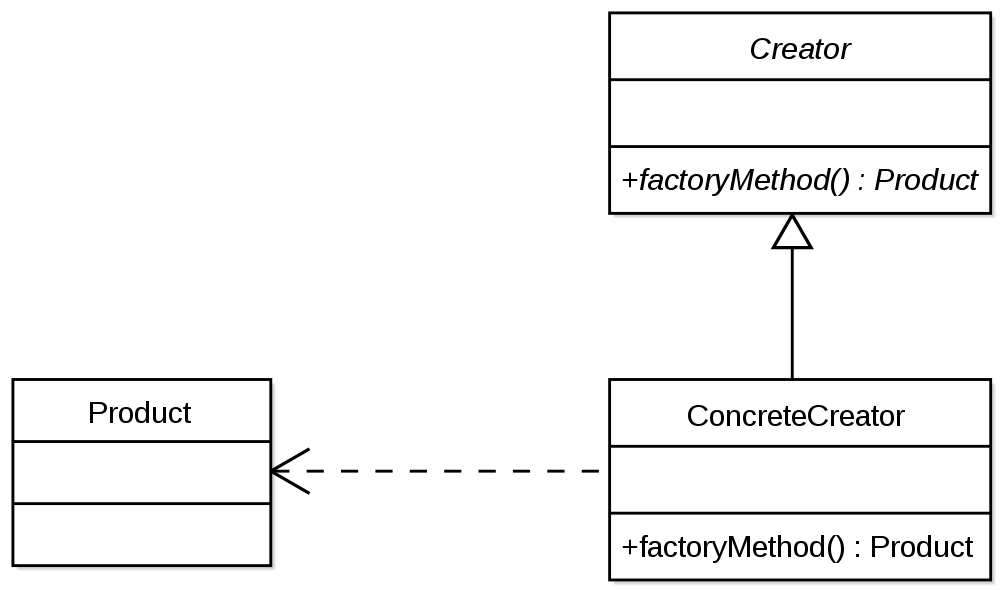
\includegraphics[width=.9\textwidth]{1000px-FactoryMethod.png}
      \end{figure}
    \end{column}
  \end{columns}

\end{frame}

\begin{frame}{Abstract Factory}
\begin{block}{Features:}
  \begin{itemize}
    \item<1-> create product from families of products
    \item<2-> client uses abstract classes (dependency inversion)
    \item<3-> client is isolated from concrete product
    \item<4-> subclasses decide what class to instantiate
    \item<5-> easy change of family on client side
    \item<6-> consistency among products
    \item<7-> uses Factory Method to create products
    \item<8-> uses object composition
  \end{itemize}
\end{block}
\uncover<9->{
  \begin{block}{Drawbacks:}
    \begin{itemize}
      \item adding new product-family is cumbersome
        \begin{itemize}
          \item[$\Rightarrow$] abstract factory class must change
            \uncover<9->{
              \begin{itemize}
                \item[$\Rightarrow$] concrete factory classes must follow the change
              \end{itemize}
            }
        \end{itemize}
    \end{itemize}
  \end{block}
}
\end{frame}

\begin{frame}{Abstract Factory}
\begin{figure}[t]
  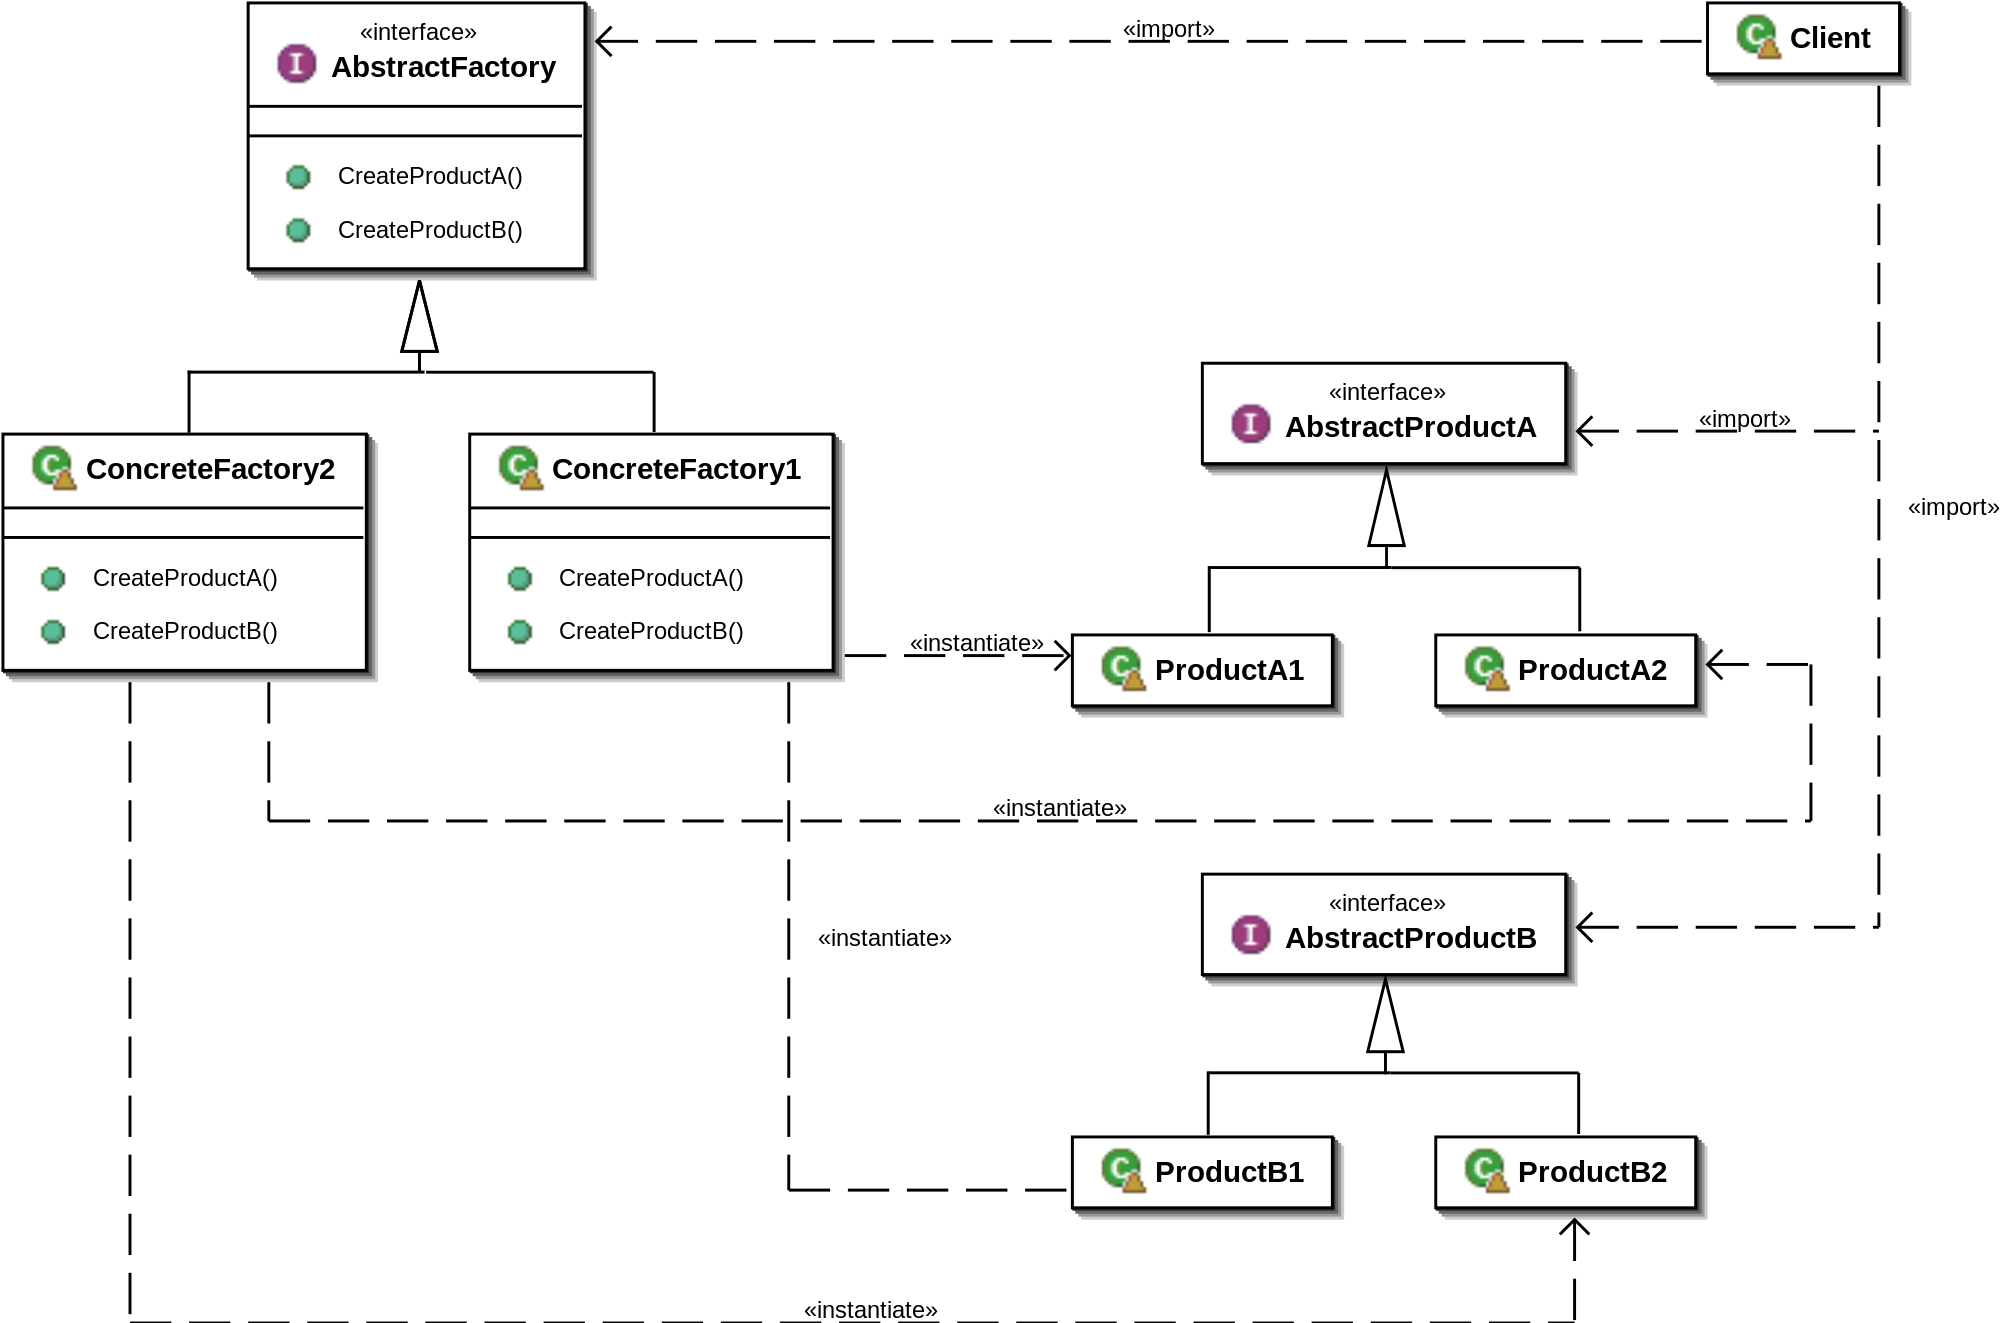
\includegraphics[width=.9\textwidth]{2000px-Abstract_factory_UML.png}
\end{figure}
\end{frame}

\begin{frame}{Object Factory}
  \begin{columns}
    \begin{column}{.47\textwidth}
      \begin{block}{Features:}
        \begin{itemize}
          \item each product has to register
          \item uses the priority inversion principle
          \item one family of product
        \end{itemize}
      \end{block}
      \uncover<2->{
        \begin{block}{Cloning:}
          \begin{itemize}
            \item make use of covariant return type
            \item common mistake: forgetting to implement $\_Clone\_$
          \end{itemize}
        \end{block}
      }
    \end{column}
    \begin{column}{.47\textwidth}
      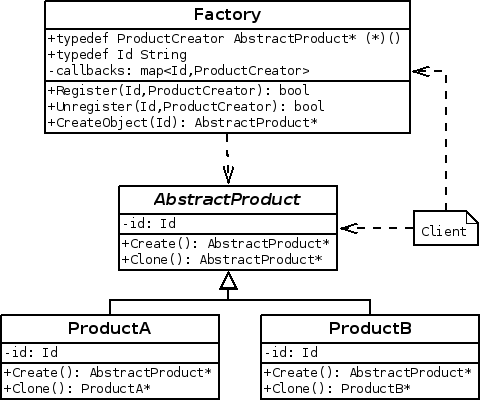
\includegraphics[width=\textwidth]{ObjFact.png}
      %\resizebox{\textwidth}{!}{ % Tikz replaces '<' with ';'
        %% Graphic for TeX using PGF
% Title: /home/attila/work/DesignPatterns/arm/ObjFact.dia
% Creator: Dia v0.97.2
% CreationDate: Fri Mar  7 22:13:09 2014
% For: attila
% \usepackage{tikz}
% The following commands are not supported in PSTricks at present
% We define them conditionally, so when they are implemented,
% this pgf file will use them.
\ifx\du\undefined
  \newlength{\du}
\fi
\setlength{\du}{15\unitlength}
\begin{tikzpicture}
\pgftransformxscale{1.000000}
\pgftransformyscale{-1.000000}
\definecolor{dialinecolor}{rgb}{0.000000, 0.000000, 0.000000}
\pgfsetstrokecolor{dialinecolor}
\definecolor{dialinecolor}{rgb}{1.000000, 1.000000, 1.000000}
\pgfsetfillcolor{dialinecolor}
\pgfsetlinewidth{0.100000\du}
\pgfsetdash{}{0pt}
\definecolor{dialinecolor}{rgb}{1.000000, 1.000000, 1.000000}
\pgfsetfillcolor{dialinecolor}
\fill (27.315300\du,-4.194410\du)--(27.315300\du,-2.794410\du)--(45.525300\du,-2.794410\du)--(45.525300\du,-4.194410\du)--cycle;
\definecolor{dialinecolor}{rgb}{0.000000, 0.000000, 0.000000}
\pgfsetstrokecolor{dialinecolor}
\draw (27.315300\du,-4.194410\du)--(27.315300\du,-2.794410\du)--(45.525300\du,-2.794410\du)--(45.525300\du,-4.194410\du)--cycle;
% setfont left to latex
\definecolor{dialinecolor}{rgb}{0.000000, 0.000000, 0.000000}
\pgfsetstrokecolor{dialinecolor}
\node at (36.420300\du,-3.244410\du){Factory};
\definecolor{dialinecolor}{rgb}{1.000000, 1.000000, 1.000000}
\pgfsetfillcolor{dialinecolor}
\fill (27.315300\du,-2.794410\du)--(27.315300\du,-0.194410\du)--(45.525300\du,-0.194410\du)--(45.525300\du,-2.794410\du)--cycle;
\definecolor{dialinecolor}{rgb}{0.000000, 0.000000, 0.000000}
\pgfsetstrokecolor{dialinecolor}
\draw (27.315300\du,-2.794410\du)--(27.315300\du,-0.194410\du)--(45.525300\du,-0.194410\du)--(45.525300\du,-2.794410\du)--cycle;
% setfont left to latex
\definecolor{dialinecolor}{rgb}{0.000000, 0.000000, 0.000000}
\pgfsetstrokecolor{dialinecolor}
\node[anchor=west] at (27.465300\du,-2.094410\du){+typedef ProductCreator AbstractProduct* (*)()};
% setfont left to latex
\definecolor{dialinecolor}{rgb}{0.000000, 0.000000, 0.000000}
\pgfsetstrokecolor{dialinecolor}
\node[anchor=west] at (27.465300\du,-1.294410\du){+typedef Id String};
% setfont left to latex
\definecolor{dialinecolor}{rgb}{0.000000, 0.000000, 0.000000}
\pgfsetstrokecolor{dialinecolor}
\node[anchor=west] at (27.465300\du,-0.494410\du){-callbacks: map$<$Id,ProductCreator$>$};
\definecolor{dialinecolor}{rgb}{1.000000, 1.000000, 1.000000}
\pgfsetfillcolor{dialinecolor}
\fill (27.315300\du,-0.194410\du)--(27.315300\du,2.405590\du)--(45.525300\du,2.405590\du)--(45.525300\du,-0.194410\du)--cycle;
\definecolor{dialinecolor}{rgb}{0.000000, 0.000000, 0.000000}
\pgfsetstrokecolor{dialinecolor}
\draw (27.315300\du,-0.194410\du)--(27.315300\du,2.405590\du)--(45.525300\du,2.405590\du)--(45.525300\du,-0.194410\du)--cycle;
% setfont left to latex
\definecolor{dialinecolor}{rgb}{0.000000, 0.000000, 0.000000}
\pgfsetstrokecolor{dialinecolor}
\node[anchor=west] at (27.465300\du,0.505590\du){+Register(Id,ProductCreator): bool};
% setfont left to latex
\definecolor{dialinecolor}{rgb}{0.000000, 0.000000, 0.000000}
\pgfsetstrokecolor{dialinecolor}
\node[anchor=west] at (27.465300\du,1.305590\du){+Unregister(Id,ProductCreator): bool};
% setfont left to latex
\definecolor{dialinecolor}{rgb}{0.000000, 0.000000, 0.000000}
\pgfsetstrokecolor{dialinecolor}
\node[anchor=west] at (27.465300\du,2.105590\du){+CreateObject(Id): AbstractProduct*};
\pgfsetlinewidth{0.100000\du}
\pgfsetdash{}{0pt}
\definecolor{dialinecolor}{rgb}{1.000000, 1.000000, 1.000000}
\pgfsetfillcolor{dialinecolor}
\fill (31.000000\du,5.050000\du)--(31.000000\du,6.450000\du)--(41.895000\du,6.450000\du)--(41.895000\du,5.050000\du)--cycle;
\definecolor{dialinecolor}{rgb}{0.000000, 0.000000, 0.000000}
\pgfsetstrokecolor{dialinecolor}
\draw (31.000000\du,5.050000\du)--(31.000000\du,6.450000\du)--(41.895000\du,6.450000\du)--(41.895000\du,5.050000\du)--cycle;
% setfont left to latex
\definecolor{dialinecolor}{rgb}{0.000000, 0.000000, 0.000000}
\pgfsetstrokecolor{dialinecolor}
\node at (36.447500\du,6.000000\du){AbstractProduct};
\definecolor{dialinecolor}{rgb}{1.000000, 1.000000, 1.000000}
\pgfsetfillcolor{dialinecolor}
\fill (31.000000\du,6.450000\du)--(31.000000\du,7.450000\du)--(41.895000\du,7.450000\du)--(41.895000\du,6.450000\du)--cycle;
\definecolor{dialinecolor}{rgb}{0.000000, 0.000000, 0.000000}
\pgfsetstrokecolor{dialinecolor}
\draw (31.000000\du,6.450000\du)--(31.000000\du,7.450000\du)--(41.895000\du,7.450000\du)--(41.895000\du,6.450000\du)--cycle;
% setfont left to latex
\definecolor{dialinecolor}{rgb}{0.000000, 0.000000, 0.000000}
\pgfsetstrokecolor{dialinecolor}
\node[anchor=west] at (31.150000\du,7.150000\du){-id: Id};
\definecolor{dialinecolor}{rgb}{1.000000, 1.000000, 1.000000}
\pgfsetfillcolor{dialinecolor}
\fill (31.000000\du,7.450000\du)--(31.000000\du,8.450000\du)--(41.895000\du,8.450000\du)--(41.895000\du,7.450000\du)--cycle;
\definecolor{dialinecolor}{rgb}{0.000000, 0.000000, 0.000000}
\pgfsetstrokecolor{dialinecolor}
\draw (31.000000\du,7.450000\du)--(31.000000\du,8.450000\du)--(41.895000\du,8.450000\du)--(41.895000\du,7.450000\du)--cycle;
% setfont left to latex
\definecolor{dialinecolor}{rgb}{0.000000, 0.000000, 0.000000}
\pgfsetstrokecolor{dialinecolor}
\node[anchor=west] at (31.150000\du,8.150000\du){+Create(): AbstractProduct*};
\pgfsetlinewidth{0.100000\du}
\pgfsetdash{}{0pt}
\definecolor{dialinecolor}{rgb}{1.000000, 1.000000, 1.000000}
\pgfsetfillcolor{dialinecolor}
\fill (25.100000\du,11.500000\du)--(25.100000\du,12.900000\du)--(35.995000\du,12.900000\du)--(35.995000\du,11.500000\du)--cycle;
\definecolor{dialinecolor}{rgb}{0.000000, 0.000000, 0.000000}
\pgfsetstrokecolor{dialinecolor}
\draw (25.100000\du,11.500000\du)--(25.100000\du,12.900000\du)--(35.995000\du,12.900000\du)--(35.995000\du,11.500000\du)--cycle;
% setfont left to latex
\definecolor{dialinecolor}{rgb}{0.000000, 0.000000, 0.000000}
\pgfsetstrokecolor{dialinecolor}
\node at (30.547500\du,12.450000\du){ProductA};
\definecolor{dialinecolor}{rgb}{1.000000, 1.000000, 1.000000}
\pgfsetfillcolor{dialinecolor}
\fill (25.100000\du,12.900000\du)--(25.100000\du,13.900000\du)--(35.995000\du,13.900000\du)--(35.995000\du,12.900000\du)--cycle;
\definecolor{dialinecolor}{rgb}{0.000000, 0.000000, 0.000000}
\pgfsetstrokecolor{dialinecolor}
\draw (25.100000\du,12.900000\du)--(25.100000\du,13.900000\du)--(35.995000\du,13.900000\du)--(35.995000\du,12.900000\du)--cycle;
% setfont left to latex
\definecolor{dialinecolor}{rgb}{0.000000, 0.000000, 0.000000}
\pgfsetstrokecolor{dialinecolor}
\node[anchor=west] at (25.250000\du,13.600000\du){-id: Id};
\definecolor{dialinecolor}{rgb}{1.000000, 1.000000, 1.000000}
\pgfsetfillcolor{dialinecolor}
\fill (25.100000\du,13.900000\du)--(25.100000\du,14.900000\du)--(35.995000\du,14.900000\du)--(35.995000\du,13.900000\du)--cycle;
\definecolor{dialinecolor}{rgb}{0.000000, 0.000000, 0.000000}
\pgfsetstrokecolor{dialinecolor}
\draw (25.100000\du,13.900000\du)--(25.100000\du,14.900000\du)--(35.995000\du,14.900000\du)--(35.995000\du,13.900000\du)--cycle;
% setfont left to latex
\definecolor{dialinecolor}{rgb}{0.000000, 0.000000, 0.000000}
\pgfsetstrokecolor{dialinecolor}
\node[anchor=west] at (25.250000\du,14.600000\du){+Create(): AbstractProduct*};
\pgfsetlinewidth{0.100000\du}
\pgfsetdash{}{0pt}
\definecolor{dialinecolor}{rgb}{1.000000, 1.000000, 1.000000}
\pgfsetfillcolor{dialinecolor}
\fill (38.100000\du,11.500000\du)--(38.100000\du,12.900000\du)--(48.995000\du,12.900000\du)--(48.995000\du,11.500000\du)--cycle;
\definecolor{dialinecolor}{rgb}{0.000000, 0.000000, 0.000000}
\pgfsetstrokecolor{dialinecolor}
\draw (38.100000\du,11.500000\du)--(38.100000\du,12.900000\du)--(48.995000\du,12.900000\du)--(48.995000\du,11.500000\du)--cycle;
% setfont left to latex
\definecolor{dialinecolor}{rgb}{0.000000, 0.000000, 0.000000}
\pgfsetstrokecolor{dialinecolor}
\node at (43.547500\du,12.450000\du){ProductB};
\definecolor{dialinecolor}{rgb}{1.000000, 1.000000, 1.000000}
\pgfsetfillcolor{dialinecolor}
\fill (38.100000\du,12.900000\du)--(38.100000\du,13.900000\du)--(48.995000\du,13.900000\du)--(48.995000\du,12.900000\du)--cycle;
\definecolor{dialinecolor}{rgb}{0.000000, 0.000000, 0.000000}
\pgfsetstrokecolor{dialinecolor}
\draw (38.100000\du,12.900000\du)--(38.100000\du,13.900000\du)--(48.995000\du,13.900000\du)--(48.995000\du,12.900000\du)--cycle;
% setfont left to latex
\definecolor{dialinecolor}{rgb}{0.000000, 0.000000, 0.000000}
\pgfsetstrokecolor{dialinecolor}
\node[anchor=west] at (38.250000\du,13.600000\du){-id: Id};
\definecolor{dialinecolor}{rgb}{1.000000, 1.000000, 1.000000}
\pgfsetfillcolor{dialinecolor}
\fill (38.100000\du,13.900000\du)--(38.100000\du,14.900000\du)--(48.995000\du,14.900000\du)--(48.995000\du,13.900000\du)--cycle;
\definecolor{dialinecolor}{rgb}{0.000000, 0.000000, 0.000000}
\pgfsetstrokecolor{dialinecolor}
\draw (38.100000\du,13.900000\du)--(38.100000\du,14.900000\du)--(48.995000\du,14.900000\du)--(48.995000\du,13.900000\du)--cycle;
% setfont left to latex
\definecolor{dialinecolor}{rgb}{0.000000, 0.000000, 0.000000}
\pgfsetstrokecolor{dialinecolor}
\node[anchor=west] at (38.250000\du,14.600000\du){+Create(): AbstractProduct*};
\pgfsetlinewidth{0.100000\du}
\pgfsetdash{}{0pt}
\pgfsetmiterjoin
\pgfsetbuttcap
{
\definecolor{dialinecolor}{rgb}{0.000000, 0.000000, 0.000000}
\pgfsetfillcolor{dialinecolor}
% was here!!!
\definecolor{dialinecolor}{rgb}{0.000000, 0.000000, 0.000000}
\pgfsetstrokecolor{dialinecolor}
\draw (36.447500\du,8.500427\du)--(36.447500\du,10.375000\du)--(30.547500\du,10.375000\du)--(30.547500\du,11.449573\du);
}
\definecolor{dialinecolor}{rgb}{0.000000, 0.000000, 0.000000}
\pgfsetstrokecolor{dialinecolor}
\draw (36.447500\du,9.412231\du)--(36.447500\du,10.375000\du)--(30.547500\du,10.375000\du)--(30.547500\du,11.449573\du);
\pgfsetmiterjoin
\definecolor{dialinecolor}{rgb}{1.000000, 1.000000, 1.000000}
\pgfsetfillcolor{dialinecolor}
\fill (36.847500\du,9.412231\du)--(36.447500\du,8.612231\du)--(36.047500\du,9.412231\du)--cycle;
\pgfsetlinewidth{0.100000\du}
\pgfsetdash{}{0pt}
\pgfsetmiterjoin
\definecolor{dialinecolor}{rgb}{0.000000, 0.000000, 0.000000}
\pgfsetstrokecolor{dialinecolor}
\draw (36.847500\du,9.412231\du)--(36.447500\du,8.612231\du)--(36.047500\du,9.412231\du)--cycle;
% setfont left to latex
\pgfsetlinewidth{0.100000\du}
\pgfsetdash{}{0pt}
\pgfsetmiterjoin
\pgfsetbuttcap
{
\definecolor{dialinecolor}{rgb}{0.000000, 0.000000, 0.000000}
\pgfsetfillcolor{dialinecolor}
% was here!!!
\definecolor{dialinecolor}{rgb}{0.000000, 0.000000, 0.000000}
\pgfsetstrokecolor{dialinecolor}
\draw (36.447500\du,8.450000\du)--(36.447500\du,10.375000\du)--(43.547500\du,10.375000\du)--(43.547500\du,11.500000\du);
}
\definecolor{dialinecolor}{rgb}{0.000000, 0.000000, 0.000000}
\pgfsetstrokecolor{dialinecolor}
\draw (36.447500\du,9.361803\du)--(36.447500\du,10.375000\du)--(43.547500\du,10.375000\du)--(43.547500\du,11.500000\du);
\pgfsetmiterjoin
\definecolor{dialinecolor}{rgb}{1.000000, 1.000000, 1.000000}
\pgfsetfillcolor{dialinecolor}
\fill (36.847500\du,9.361803\du)--(36.447500\du,8.561803\du)--(36.047500\du,9.361803\du)--cycle;
\pgfsetlinewidth{0.100000\du}
\pgfsetdash{}{0pt}
\pgfsetmiterjoin
\definecolor{dialinecolor}{rgb}{0.000000, 0.000000, 0.000000}
\pgfsetstrokecolor{dialinecolor}
\draw (36.847500\du,9.361803\du)--(36.447500\du,8.561803\du)--(36.047500\du,9.361803\du)--cycle;
% setfont left to latex
\pgfsetlinewidth{0.100000\du}
\pgfsetdash{}{0pt}
\definecolor{dialinecolor}{rgb}{1.000000, 1.000000, 1.000000}
\pgfsetfillcolor{dialinecolor}
\fill (45.682188\du,5.881272\du)--(48.292188\du,5.881272\du)--(48.892188\du,6.481272\du)--(48.892188\du,7.581272\du)--(45.682188\du,7.581272\du)--cycle;
\definecolor{dialinecolor}{rgb}{0.000000, 0.000000, 0.000000}
\pgfsetstrokecolor{dialinecolor}
\draw (45.682188\du,5.881272\du)--(48.292188\du,5.881272\du)--(48.892188\du,6.481272\du)--(48.892188\du,7.581272\du)--(45.682188\du,7.581272\du)--cycle;
\pgfsetlinewidth{0.050000\du}
\definecolor{dialinecolor}{rgb}{0.000000, 0.000000, 0.000000}
\pgfsetstrokecolor{dialinecolor}
\draw (48.292188\du,5.881272\du)--(48.292188\du,6.481272\du)--(48.892188\du,6.481272\du);
% setfont left to latex
\definecolor{dialinecolor}{rgb}{0.000000, 0.000000, 0.000000}
\pgfsetstrokecolor{dialinecolor}
\node[anchor=west] at (46.032188\du,7.126272\du){Client};
\pgfsetlinewidth{0.100000\du}
\pgfsetdash{{1.000000\du}{1.000000\du}}{0\du}
\pgfsetdash{{0.400000\du}{0.400000\du}}{0\du}
\pgfsetmiterjoin
\pgfsetbuttcap
{
\definecolor{dialinecolor}{rgb}{0.000000, 0.000000, 0.000000}
\pgfsetfillcolor{dialinecolor}
% was here!!!
\pgfsetarrowsend{to}
\definecolor{dialinecolor}{rgb}{0.000000, 0.000000, 0.000000}
\pgfsetstrokecolor{dialinecolor}
\draw (36.420300\du,2.455999\du)--(36.420300\du,3.527786\du)--(36.447500\du,3.527786\du)--(36.447500\du,4.999573\du);
}
% setfont left to latex
\pgfsetlinewidth{0.100000\du}
\pgfsetdash{{0.400000\du}{0.400000\du}}{0\du}
\pgfsetdash{{0.400000\du}{0.400000\du}}{0\du}
\pgfsetmiterjoin
\pgfsetbuttcap
{
\definecolor{dialinecolor}{rgb}{0.000000, 0.000000, 0.000000}
\pgfsetfillcolor{dialinecolor}
% was here!!!
\pgfsetarrowsend{to}
\definecolor{dialinecolor}{rgb}{0.000000, 0.000000, 0.000000}
\pgfsetstrokecolor{dialinecolor}
\draw (45.631784\du,6.731272\du)--(43.988560\du,6.731272\du)--(43.988560\du,6.750000\du)--(41.945336\du,6.750000\du);
}
% setfont left to latex
\pgfsetlinewidth{0.100000\du}
\pgfsetdash{{0.400000\du}{0.400000\du}}{0\du}
\pgfsetdash{{0.400000\du}{0.400000\du}}{0\du}
\pgfsetmiterjoin
\pgfsetbuttcap
{
\definecolor{dialinecolor}{rgb}{0.000000, 0.000000, 0.000000}
\pgfsetfillcolor{dialinecolor}
% was here!!!
\pgfsetarrowsend{to}
\definecolor{dialinecolor}{rgb}{0.000000, 0.000000, 0.000000}
\pgfsetstrokecolor{dialinecolor}
\draw (47.287188\du,5.881272\du)--(47.287188\du,-0.694410\du)--(45.525300\du,-0.694410\du);
}
% setfont left to latex
\end{tikzpicture}

      %}
    \end{column}
  \end{columns}
\end{frame}

\begin{frame}{Resources}
\begin{itemize}
  \item Design Patterns: Elements of Reusable Object-Oriented Software\\
    \small{\textit{"Gang of Four"}}
  \item Modern C++ Design: Generic Programming and Design Patterns Applied\\
    \small{\textit{Andrei Alexandrescu}}
  \item Head First: Design Patterns \\
    \small{\textit{Eric Freeman \& Elisabeth Freeman}}
\end{itemize}
\end{frame}

\begin{frame}
  \only<1>{
    \begin{center}
      \Huge{Questions?}
    \end{center}
  }
  \only<2>{
    \begin{center}
      \Huge{Thank You!}
    \end{center}
  }
\end{frame}

\end{document}
